\chapter{Zapojení GPIO pinů na Raspberry Pi}
\begin{table}[h]
\centering
\caption{Zapojení GPIO pinů na Raspberry Pi}
\label{gpio}
\begin{tabular}{|l|l|l|l|l|l|l|l|}
\hline
\textbf{zapojení} & \textbf{název} & \textbf{BCM} & \textbf{pin} & \textbf{pin} & \textbf{BCM} & \textbf{název} & \textbf{zapojení} \\ \hline
-                 & 3v3            & -            & 1            & 2            & -            & 5V             & Napájení                \\ \hline
-                 & SDA            & 2            & 3            & 4            & -            & 5V             & -                 \\ \hline
 Tlačítko ON/OFF  & SCL            & 3            & 5            & 6            & -            & GND            & GND                 \\ \hline
 SIM800 RST       & GPCLK0         & 4            & 7            & 8            & 14           & TXD            & SIM800 Rx         \\ \hline
-                 & GND            & -            & 9            & 10           & 15           & RXD            & SIM800 Tx         \\ \hline
-                 &                & 17           & 11           & 12           & 18           & PWM0           & PIR signál        \\ \hline
-                 &                & 27           & 13           & 14           & -            & GND            & -                 \\ \hline
-                 &                & 22           & 15           & 16           & 23           &                & LED signál        \\ \hline
-                 & 3v3            & -            & 17           & 18           & 24           &                & -                 \\ \hline
-                 & MOSI           & 10           & 19           & 20           & -            & GND            & -                 \\ \hline
-                 & MISO           & 9            & 21           & 22           & 25           &                & -                 \\ \hline
-                 & SCLK           & 11           & 23           & 24           & 8            & CE0            & -                  \\ \hline
-                 & GND            & -            & 25           & 26           & 7            & CE1            & -                  \\ \hline
-                 & ID\_SD         & 0            & 27           & 28           & 1            & ID\_SC         & -                 \\ \hline
-                 &                & 5            & 29           & 30           & -            & GND            & -                 \\ \hline
-                 &                & 6            & 31           & 32           & 12           & PWM0           & -                 \\ \hline
-                 & PWM1           & 13           & 33           & 34           & -            & GND            & -                 \\ \hline
-                 & MISO           & 19           & 35           & 36           & 16           &                & -                  \\ \hline
-                 &                & 26           & 37           & 38           & 20           & MOSI           & -                  \\ \hline
-                 & GND            & -            & 39           & 40           & 21           & SCLK           & -                 \\ \hline
\end{tabular}
\end{table}

\chapter{Denní úhrn solárního záření v Brně}
\begin{figure}[!h]
  \begin{center}
    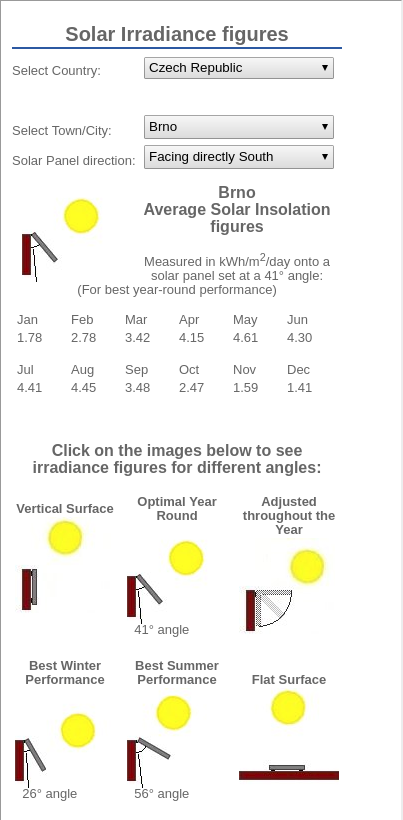
\includegraphics[scale=0.61]{obrazky/solar-irradiance-Brno.png}
  \end{center}
  \caption{Solar Irradiance Brno \cite{solar}}
\end{figure}


\chapter{Dokumentace aplikace}
